\section{Eigenkapitalfinanzierung, Aktien}

\textbf{Unterschiede Eigen- und Fremdkapital}:
\begin{center}
	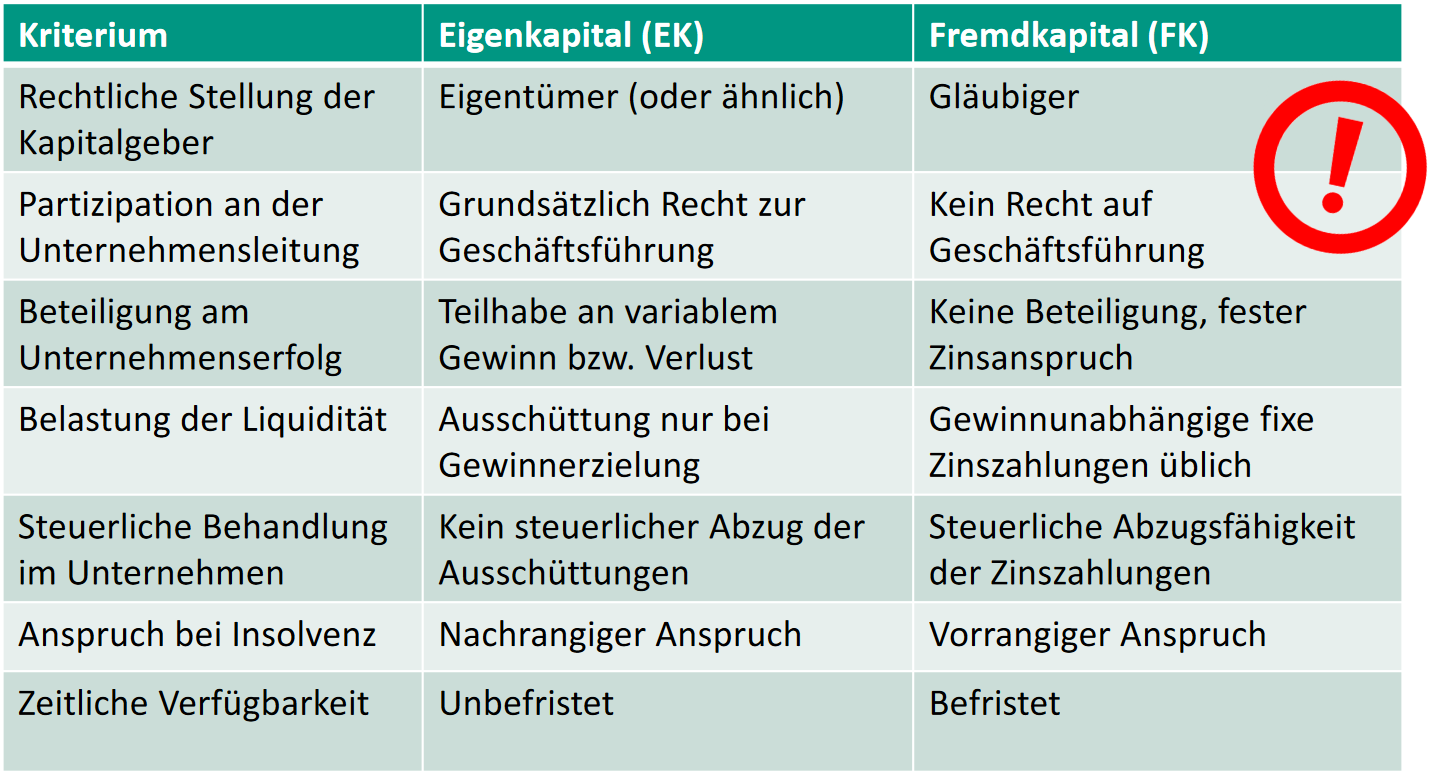
\includegraphics[width=0.8\textwidth]{images/ef-capital.png}
\end{center}

\textbf{Aktien}: Grundkapital einer Aktiengesellschaft wird in Aktien aufgeteilt und bildet neben Gewinnrücklagen das Eigenkapital. 
Diese können gehandelt werden und besitzen keine begrenzte Laufzeit.

\textbf{Stammaktien}:
\begin{itemize}
	\item Recht auf Anteil am Bilanzgewinn (\textbf{Dividende})
	\item Recht auf Anteil am Liquidationserlös
	\item Teilnahme, Rederecht, Stimmrecht auf Hauptversammlung
	\item Recht zur Stellung von Anträgen
	\item Auskunftsrecht
	\item Recht auf Bezug junger Aktien
\end{itemize}
\bigskip
\textbf{Vorzugsaktien}: Bestimmte Rechte kommen hinzu oder fallen weg (z.B. höhere Dividenden, mehr/weniger Stimmen)\\

\textbf{Kapitalbeschaffung durch Börsengang} (IPO, Initial Public Offering):
\begin{center}
	\includegraphics[width=0.75\textwidth]{images/börsengang.png}
\end{center}

\textbf{IPO-Phänomene}:
\begin{itemize}
	\item \textbf{Underpricing}: Bookbuildingpreis liegt meist deutlich unter dem ersten Handelskurs
	\item \textbf{Zyklizität}: Viele (wenige) IPOs in ökonomisch guten (schlechten) Zeiten
	\item \textbf{Kosten des Börsengangs}: Hohe Transaktionskosten für Unternehmen
	\item \textbf{Langfrist-Performance}: 3-5 Jahre nach IPO fällt meist eher durchschnittlich aus
\end{itemize}
\bigskip
\textbf{Kapitalbeschaffung durch Kapitalerhöhung}:
\begin{itemize}
	\item \textbf{Ordentliche Kapitalerhöhung}: Ausgabe von jungen Aktien zur Beschaffung neuen Eigenkapitals
	\item \textbf{Bedingte Kapitalerhöhung}: Kapitalerhöhung durch Umtausch-/Bezugsrecht\\ $\rightarrow$ Höhe ungewiss
	\item \textbf{Genehmigtes Kapital}: Ermächtigung des Vorstandes Eigenkapital zu emittieren, Kapital kann innerhalb dieses Zeitraums ohne Hauptversammlung erhöht werden 
	$\rightarrow$ Zeitpunkt ungewiss
\end{itemize}
\bigskip
\textbf{Auswirkung der Dividendenzahlung auf Aktienkurs}:
\begin{itemize}
	\item Aktienkurs sinkt um die ausgezahlte Dividende
	\item nicht von der Steuer absetzbar
	\item keine Zahlungsverpflichtung, können also nicht zur Insolvenz führen
\end{itemize}
\bigskip
\textbf{Tendenz zur Glättung von Dividenden im Zeitablauf}:
\begin{itemize}
	\item Dividenden haben \enquote{verbindlichen} Charakter gegenüber Aktionären\\
	$\rightarrow$ Führt zu langfristig möglichst stabilen Dividenden (\textbf{Dividend smoothing})
	\item \textbf{Signalwirkungen}:
	\begin{itemize}
		\item Dividendenerhöhung $\rightarrow$ Positive Zukunftserwartungen $\rightarrow$ Positive Aktienkursveränderung
		\item Dividendensenkung $\rightarrow$ Negative Zukunftserwartungen $\rightarrow$ Negative Aktienkursveränderung
		\item \textbf{Vorsicht}: Ausnahmen möglich!
	\end{itemize}
\end{itemize}
\bigskip
\textbf{Einfluss von Steuerpräferenzen von Investoren}:
\begin{itemize}
	\item Dividenden sind häufig mit einem höheren Steuersatz belegt als Kapitalgewinne
	\item Besteuerung kann je nach Investorentyp variieren
	\item \textbf{Dividend puzzle}: Dividenden bleiben aber trotz ihres steuerlichen Nachteils ein verwendetes Mittel der Ausschüttungspolitik
	\item \textbf{Klienteleffekt}: Unternehmen passt Dividendenpolitik den Steuerpräferenzen der Aktionäre an
	\item \textbf{Steuerarbitrage}: Zunehmendes Handelsvolumen um den Ex-Dividenden-Termin, da niedrig besteuerte Investoren davor kaufen und hinterher wieder verkaufen
\end{itemize}